\documentclass[sigconf]{acmart}

\usepackage{booktabs} % For formal tables

\acmPrice{15.00}

% The next six lines come directly from the completed rights form.
% You MUST replace them with the lines specific to your accepted work.
\copyrightyear{2017}
\acmYear{2017}
\setcopyright{rightsretained}
\acmConference{Conference Name}{Conference Date and Year}{Conference Location}
\acmDOI{10.1145/8888888.7777777}
\acmISBN{978-1-4503-1234-5/17/07}

% Use the "authoryear" citation style, and make sure citations are in [square brackets].
\citestyle{acmauthoryear}
\setcitestyle{square}

% A useful command for controlling the number of authors per row.
% The default value of "authorsperrow" is 2.
\settopmatter{authorsperrow=4}

% end of preamble.

\begin{document}

% Title. 
% If your title is long, consider \title[short title]{full title} - "short title" will be used for running heads.
\title{Preparing Your Article or Abstract}

% Authors.
\author{John DeJohnette}
\affiliation{%
  \department{Department of Computer Science and Engineering}
  \institution{University of Minnesota}}
\email{johnd@umn.edu}

\author{Brittany Rowland-Smith}
\affiliation{%
  \institution{St. Olaf College}}
\email{br-s@gmail.com}

\author{Nicholas Badeeri}
\affiliation{%
  \institution{MathWorks, Inc.}}
\email{badeeri@mathworks.com}

\author{Andrew Joseph Foyt}
\affiliation{%
  \department{College of Engineering}
  \institution{University of Houston}}
\email{foyt_aj@uh.edu}

% This command defines the author string for running heads.
\renewcommand{\shortauthors}{DeJohnette, Rowland-Smith, Badeeri, and Foyt}

% abstract
\begin{abstract}
This formatted document contains examples of many of the elements of an abstract or technical paper, including multiple authors, CCS concepts and keywords, sections and subsections, formulae, tables, figures, enumeration environments, and citations and references. 

Of particular note to authors preparing work for publication at an event sponsored by ACM SIGGRAPH are the citations and references; although the ACM article default is for numbered citations and references, we use the ``author year'' citation and reference style.
\end{abstract}

%CCS
\begin{CCSXML}
<ccs2012>
<concept>
<concept_id>10010147.10010371.10010372</concept_id>
<concept_desc>Computing methodologies~Rendering</concept_desc>
<concept_significance>500</concept_significance>
</concept>
<concept>
<concept_id>10010147.10010371.10010372.10010374</concept_id>
<concept_desc>Computing methodologies~Ray tracing</concept_desc>
<concept_significance>500</concept_significance>
</concept>
</ccs2012>
\end{CCSXML}

\ccsdesc[500]{Computing methodologies~Rendering}
\ccsdesc[500]{Computing methodologies~Ray tracing}

%keywords
\keywords{ray tracing, global illumination, octrees, quadtrees}

% A "teaser" figure, centered below the title and authors and above the body of the work.
\begin{teaserfigure}
  \centering
  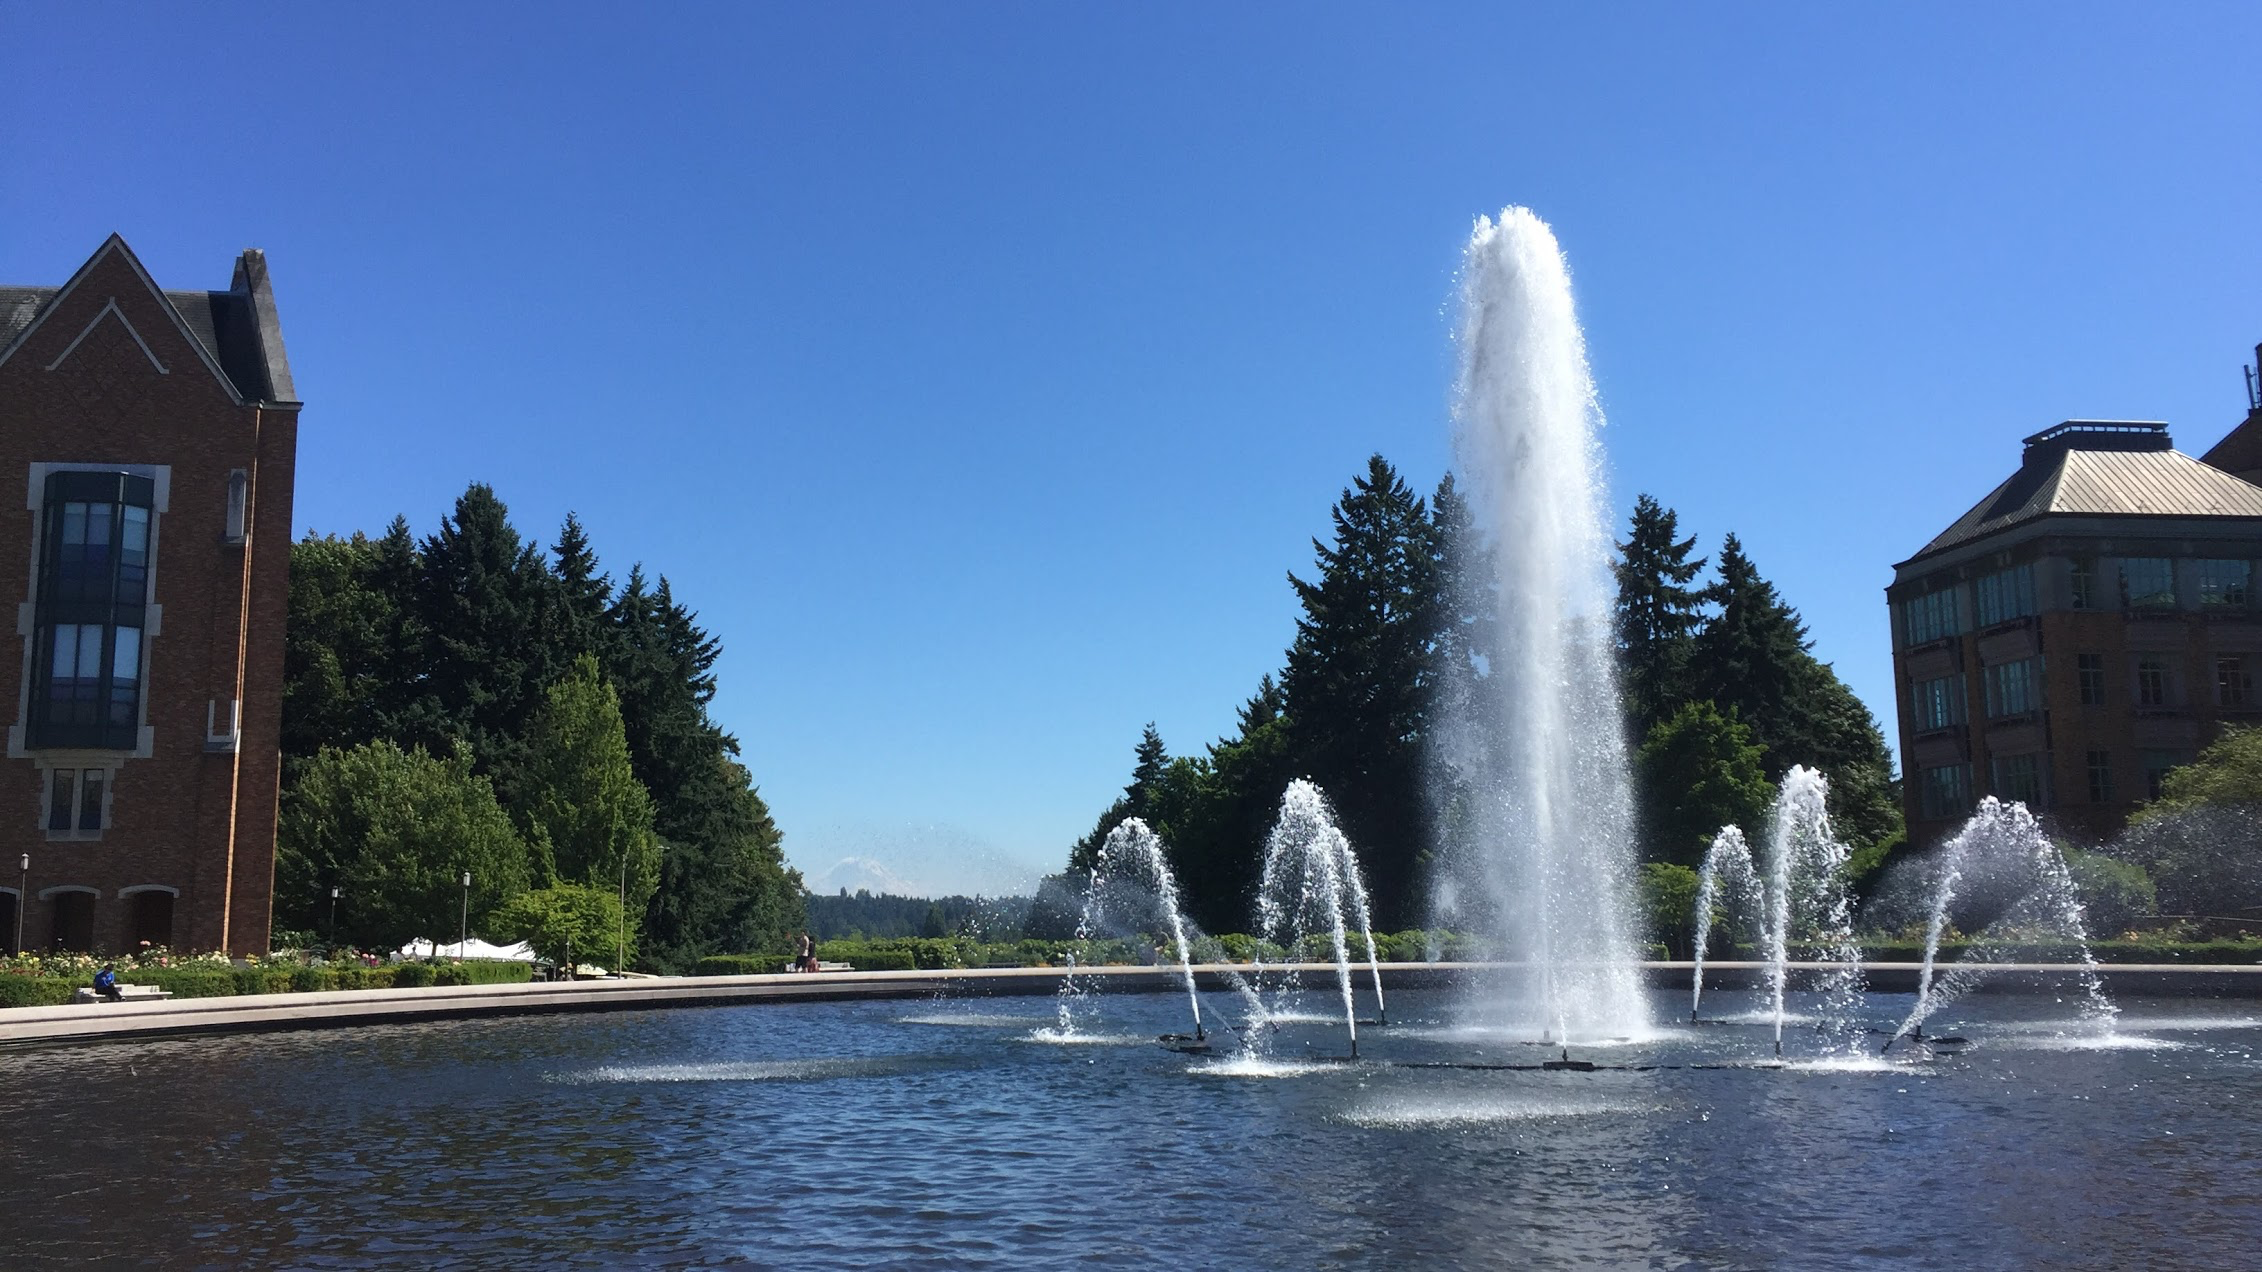
\includegraphics[width=6.0in]{aaafiles/fountain}
  \caption{Drumheller Fountain, The University of Washington, Seattle WA.}
\end{teaserfigure}

% Processes all of the front-end information and starts the body of the work.
\maketitle

\section{Introduction}

Lorem ipsum dolor sit amet, consectetur adipiscing elit. Fusce auctor accumsan nulla, vitae pharetra ipsum sagittis sit amet. \cite{Park:2006:DSI, notes2002} Donec ac metus consectetur, venenatis magna sit amet, viverra sapien. Class aptent taciti sociosqu ad litora torquent per conubia nostra, per inceptos himenaeos. Phasellus eleifend sem sit amet arcu congue tempus. Proin at iaculis orci. Pellentesque habitant morbi tristique senectus et netus et malesuada fames ac turpis egestas. Orci varius natoque penatibus et magnis dis parturient montes, nascetur ridiculus mus. \cite{Pellacini:2005:LAH} Etiam feugiat dui sit amet ante pellentesque, sed malesuada libero ornare. Curabitur tempor ligula leo, in feugiat urna ornare luctus. Fusce quis metus sit amet neque sagittis elementum. Quisque facilisis quam quis tortor volutpat, et sodales urna efficitur.

\begin{figure}[ht]
  \centering
  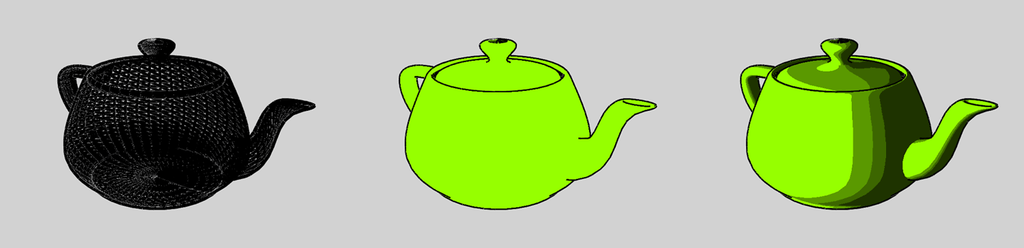
\includegraphics[width=\linewidth]{aaafiles/teapots}
  \caption{Cel-shaded teapots. Image by Nicolas Sourd [CC-BY-SA-3.0 (http://creativecommons.org/licenses/by-sa/3.0/)], via Wikimedia Commons. (\url{https://goo.gl/5e6tNk}).}
\end{figure}

Duis sagittis massa odio, consequat ornare mauris imperdiet blandit. \cite{levoy:2000:TDM} Donec vel pulvinar nisl. Nam pretium vitae risus a consectetur. \cite{sako:2001:SSB, fedkiw:2001:VSO, Jobs95} Vestibulum efficitur auctor mauris. Vestibulum nec orci suscipit, faucibus mauris vel, elementum dolor. Phasellus ornare est id commodo cursus. Lorem ipsum dolor sit amet, consectetur adipiscing elit. Donec iaculis enim urna, vitae tincidunt est dictum id. Suspendisse lobortis justo id enim ornare euismod. Fusce quis turpis rhoncus, laoreet lorem eu, porttitor enim. \cite{kartch:2000:ERA, yee:2000:SSA, parke:1996:CFA} Etiam eget tempus velit. Duis iaculis id eros et mollis. Pellentesque non magna a massa rhoncus gravida id eget ex. Donec magna risus, posuere eu velit sit amet, tincidunt cursus leo. Curabitur non ultricies turpis, at sodales sapien.

\section{Exposition}

Nullam mollis in lectus vitae tempus. Nam pellentesque tincidunt leo id dapibus. Etiam in euismod diam. \cite{ceres-solver, Asaro:1976:POT} Phasellus feugiat ante et dui rhoncus, at dictum elit vehicula. Nunc ut finibus neque. Sed vehicula tristique - as shown in Table \ref{soccer} - odio at interdum. Morbi ex lectus, porttitor vel ipsum id, scelerisque facilisis metus. Cras orci sapien, luctus in eros in, suscipit rhoncus neque. Duis pharetra elit vitae sagittis maximus. Curabitur fermentum justo massa, sed placerat odio aliquam quis. Nam facilisis hendrerit ante eget maximus. Nulla et porttitor nibh, et malesuada turpis. Suspendisse potenti. Nunc ultricies suscipit quam, eget ultrices nisi viverra vitae.

\begin{table}[ht]
\begin{center}
    \caption{Soccer, or football?}
\label{soccer}
\begin{tabular}{l*{6}{c}r}
Team              & P & W & D & L & F  & A & Pts \\
\hline
Manchester United & 6 & 4 & 0 & 2 & 10 & 5 & 12  \\
Celtic            & 6 & 3 & 0 & 3 &  8 & 9 &  9  \\
Benfica           & 6 & 2 & 1 & 3 &  7 & 8 &  7  \\
FC Copenhagen     & 6 & 2 & 1 & 3 &  5 & 8 &  7  \\
\end{tabular}
\end{center}
\end{table}

Aliquam sed vehicula neque. Praesent placerat, nisi sit amet condimentum porta, justo tellus dictum eros, quis vestibulum erat massa id sapien. Vestibulum euismod purus dolor, ornare consectetur quam egestas volutpat. Curabitur sollicitudin convallis purus ultrices facilisis. Pellentesque sollicitudin maximus orci quis rutrum. Phasellus a mauris maximus sem mollis sagittis. Vivamus sagittis faucibus tincidunt. Vivamus vel suscipit leo.

\begin{figure}[h]
  \centering
  \includegraphics[width=\linewidth]{aaafiles/franklin}
  \caption{1907 Franklin Model D roadster. Photograph by Harris \& Ewing, Inc. [Public domain], via Wikimedia Commons. (\url{https://goo.gl/VLCRBB}).}
\end{figure}

\subsubsection{Participants}

Cum sociis natoque penatibus et magnis dis parturient montes, nascetur ridiculus mus. Vivamus maximus a lectus sed dictum. Curabitur pulvinar lectus nec magna molestie consequat. Donec ligula urna, scelerisque et felis sed, euismod feugiat sem. (See equation \ref{eqn:01}.) Donec urna libero, auctor sit amet sem id, malesuada tempor risus. Morbi malesuada lobortis consequat. Aliquam lacinia quam ac tristique sodales. Class aptent taciti sociosqu ad 
\begin{equation}
\label{eqn:01}
P(t)=\frac{b^{\frac{t+1}{T+1}}-b^{\frac{t}{T+1}}}{b-1},
\end{equation}
where $t=0,{\ldots}\,,T$, and $b$ is a number greater than $1$, litora torquent per conubia nostra, per inceptos himenaeos.

\begin{multline}
\label{the-rendering-equation}
L_o(x, \omega_o, \lambda, t) = L_e(x, \omega_o, \lambda, t)  + \\
\int_{\Omega} f_r(x, \omega_i, \omega_o, \lambda, t) L_i(x, \omega_i, \lambda, t)(\omega_i \cdot n) \text{d} \omega_i
\end{multline}

Lorem ipsum dolor sit amet, consectetur adipiscing elit. Fusce auctor accumsan nulla, vitae pharetra ipsum sagittis sit amet. Donec ac metus consectetur, venenatis magna sit amet, viverra sapien. Class aptent taciti sociosqu ad litora torquent per conubia nostra, per inceptos himenaeos. Phasellus eleifend sem sit amet arcu congue tempus. Proin at iaculis orci. (See equation \ref{the-rendering-equation}.) Pellentesque habitant morbi tristique senectus et netus et malesuada fames ac turpis egestas. Orci varius natoque penatibus et magnis dis parturient montes, nascetur ridiculus mus. Etiam feugiat dui sit amet ante pellentesque, sed malesuada libero ornare. Curabitur tempor ligula leo, in feugiat urna ornare luctus. Fusce quis metus sit amet neque sagittis elementum. Quisque facilisis quam quis tortor volutpat, et sodales urna efficitur.

\section{Conclusions and Future Work}

Nullam vulputate enim ut tortor mollis pharetra. Cras pellentesque sem a accumsan malesuada. Donec at massa nisl. Sed malesuada felis id nisl maximus efficitur. In pretium metus non faucibus pulvinar. Sed pulvinar elit ultrices mauris vehicula, id ultricies purus finibus. Fusce tempus elit molestie, consequat ipsum eget, iaculis nibh. Cras tincidunt, orci in lacinia tempus, mauris leo finibus orci, vitae dignissim dui risus et odio. Sed commodo ultricies nulla, et varius velit aliquam quis. Sed efficitur, ex non facilisis dignissim, lacus orci accumsan massa, dictum facilisis arcu lacus ac leo. Sed quis tellus dictum massa egestas dapibus vel et justo. Nulla euismod lectus ut purus hendrerit porttitor. Suspendisse quis dui ligula. Proin non porta libero. Maecenas vel feugiat urna.

\begin{acks}
The authors would like to thank Dr. Yuhua Li for providing the MATLAB code of the \textit{BEPS} method.
The authors would also like to thank the anonymous referees for their valuable comments and helpful suggestions. The work is supported by the \grantsponsor{GS501100001809}{National Natural Science Foundation of China}{https://doi.org/10.13039/501100001809} under Grant No.: ~\grantnum{GS501100001809}{61273304}
21 and ~\grantnum[http://www.nnsf.cn/youngscientists]{GS501100001809}{Young Scientists' Support Program}.
\end{acks}

\bibliographystyle{ACM-Reference-Format}
\bibliography{aaatemplate}
\end{document}